\message{ !name(sumarioExecutivo.tex)}
\documentclass[10pt,a4paper]{article}
\usepackage{ifpdf}
\usepackage[utf8]{inputenc}
\usepackage[portuges]{babel}
\usepackage{float}
\usepackage{graphicx}
\usepackage{enumerate}
\usepackage{url}
\usepackage[top=2cm,left=2cm,right=2cm,bottom=2cm]{geometry}
\usepackage{parskip}

\title{Análise de métodos de seleção para algoritmos genéticos}
\author{Anderson Gonçalves Marco}
\date{}
\usepackage{amsmath}
\usepackage{array}
\newcolumntype{L}[1]{>{\raggedright\let\newline\\\arraybackslash\hspace{0pt}}m{#1}}
\newcolumntype{C}[1]{>{\centering\let\newline\\\arraybackslash\hspace{0pt}}m{#1}}
\newcolumntype{R}[1]{>{\raggedleft\let\newline\\\arraybackslash\hspace{0pt}}m{#1}}
{\renewcommand{\arraystretch}{1.4}%

\begin{document}

\message{ !name(sumarioExecutivo.tex) !offset(-3) }

\maketitle
\section{Introdução}
Problemas de otimização são importantes em diferentes áreas da ciência como a engenharia de produção, mecânica e logística. Nestes tipos de problemas tenta-se conseguir o máximo de resultado com o mínimo de recursos. Os algoritmos genéticos são extremamente importantes para  a resolução destes problemas, eles são métodos baseados na teoria da evolução de Charles Darwin. A sua principal característica é a habilidade para a resolução de diversos problemas de otimização, sem que para isto seja necessário grandes esforços para a modelagem dos problemas.

Os algoritmos genéticos, apesar da sua versatilidade, possuem ainda varias lacunas em sua formulação teórica. Entre as lacunas podem ser destacadas as taxas mutação do genes  e os métodos de seleção dos cromossomos.

Este artigo faz uma comparação entre os métodos de seleção por roleta e torneio medindo a sua taxa de eficiência. Para esta analise foi criado um cenário de otimização por algoritmos genéticos, neste cenário foi maximizado a pontuação do popular jogo de celular e computador Angry Birds. 

O ambiente do jogo Angry Birds é acessível neste trabalho através do \emph{framework} AI Birds \cite{aiBirds}, sendo assim possível criar agentes capazes de realizar o cenário proposto. 

Também foi realizada uma comparação direta entre a pontuação alcançada pelos agentes criados por ambos os métodos de seleção citados e com o agente ``burro'' que o próprio \emph{framework} do AI Birds disponibiliza.

%http://www.carlosmartins.com.br/_bizplan/bizplan05.htm
\section{Algoritmos genéticos}
Algoritmos genéticos são uma técnica da inteligencia artificial para a resolução de problemas. Eles foram primeiro descritos por  John Henry Holland (\cite{primeiroAUsarAG}) e têm como  base a teoria da evolução criada por Charles Darwin. Esta teoria diz que indivíduos mais adaptados têm mais chances de se reproduzir e assim passam suas características adiante. O que permite seres vivos mais adaptados se reproduzir é a seleção pelo ambiente natural.

Charles Darwin  propôs a teoria da seleção natural no século XIX no entanto, humanos fazem seleção artificial sobre raças de animais há milhares de anos, os adaptando para seu o próprio proposito. Como exemplo da seleção artificial feita pelos humanos pode-se destacar os cachorros que evoluíram a partir de lobos selvagens, criadores de cachorros selecionaram os lobos mais dóceis para a procriação criando os cachorros.

Os algoritmos genéticos usam uma abordagem semelhante aos criadores de animais só que aplicados a vetores de dados, estes vetores são chamados de cromossomos. Cromossomos têm genes, que são os elementos do vetor, este podem ser binários, inteiros ou números reais. A Figura \ref{fig:ExemploDeVetores} ilustra estes três tipos.\\ \\
\begin{figure}[H]
  \center
  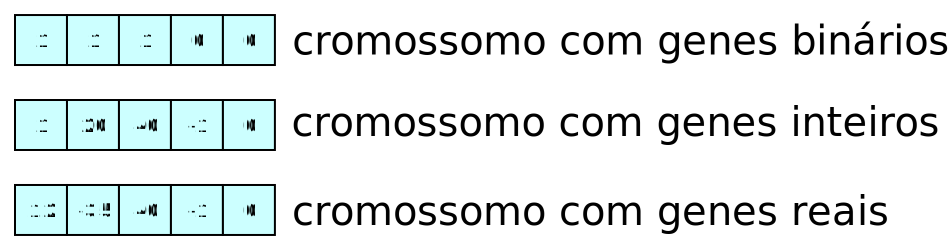
\includegraphics[scale=0.6]{imgs/tiposDeCromossomo.pdf}            
  \caption{Os vários tipos de genes que os cromossomos podem ter.}
  \label{fig:ExemploDeVetores}
\end{figure} 

A decisão sobre quais cromossomos são melhores para transmitir seus dados para as gerações futuras, o cruzamento, pertence a função que vai ser otimizada, chamada de função objetivo. A função objetivo apenas dá uma pontuação para um cromossomo que diz o quão bom ele é para a função, quem decide se o cromossomo vai ou não passar suas característica é o método de seleção. Existem dois métodos de seleção o da roleta, descrito apostila de  Diogo C. Lucas ( \cite{UFRGS-Apostila-GA}) e no livro de Almir Olivette Artero (\cite{Livro-De-IA}), e do tornei, descrito em   no livro de  Almir Olivette Artero (\cite{Livro-De-IA}) .

 Na seleção por roleta, com $N$ cromossomos, com $1 \le i \le N$, com $\vec{p}$ sendo o vetor que guarda as pontuação que cada cromossomo da geração atual recebe da função objetivo e com com $\vec{c}_i$ sendo algum cromossomo da geração atual. A possibilidade  $\vec{c}_i$ ser escolhido em cada cruzamento é de $\left [100 \left ( \frac{p_{i}}{\sum \limits_{j=i}^{n} p_{j}}\right ) \right ]\%$. 
 
 
A seleção por tornei possui varias variantes, a utilizada neste trabalho consiste em selecionar aleatoriamente quatro cromossomos da população chamados de : $\gamma_{1},\gamma_{2},\gamma_{3},\gamma_{4}$. Seleciona-se então entre $\gamma_{1}$ e $\gamma_{2}$ aquele que tem a maior pontuação este cromossomo é chamado de $\gamma_{5}$, depois seleciona-se  entre $\gamma_{3}$ e $\gamma_{4}$ aquele que tem a maior pontuação este cromossomo é chamado de $\gamma_{6}$. O cruzamento então é realizado entre $\gamma_{5}$ e $\gamma_{6}$. 


Após a escolha para os vetores existe um cruzamento entre eles. Neste cruzamento dois ou mais cromossomos, dos escolhidos, se unem para criar novos cromossomos. O número de cromossomos criados por um cruzamento geralmente igual a quantidade de cromossomos que se juntaram para o cruzamento. Existem duas principais maneiras para se fazer o cruzamento a uniforme e a por corte. \\ \\
No cruzamento por corte genes de regiões estabelecidas dos cromossomos pais, geração atual, vão para os cromossomos filhos, geração seguinte. A Figura \ref{fig:MostrandoOCruzamentoPorCorte} mostra o cruzamento por corte. 

\begin{figure}[H]
  \center
  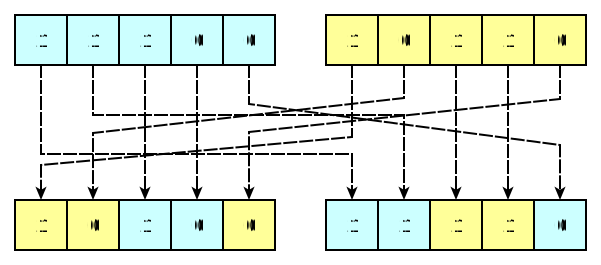
\includegraphics[scale=0.6]{imgs/diagramaCorte.pdf}            
  \caption{Cruzamento por corte entre dois cromossomos gerando dois novos cromossomos. Neste cruzamento existe dois pontos de corte.}
  \label{fig:MostrandoOCruzamentoPorCorte}
\end{figure} 

No cruzamento uniforme cada vez que um grupo de cromossomos pais se unem para formar um filho é gerada uma mascara. Esta mascara diz que genes de um determinado cromossomo pai o filho vai receber. A Figura \ref{fig:MostrandoOCruzamentoUniforme} mostra o cruzamento uniforme. 

\begin{figure}[H]
  \center
  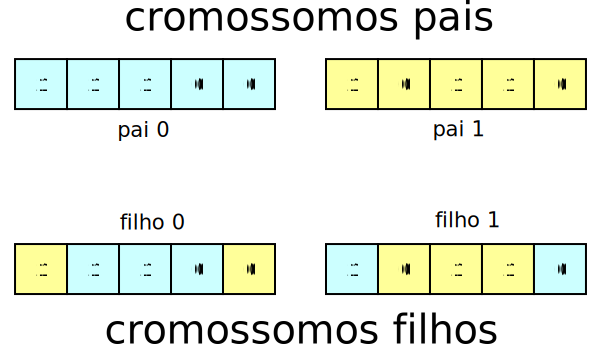
\includegraphics[scale=0.6]{imgs/diagramaMascara.pdf}            
  \caption{Cruzamento uniforme, através da mascara 10001.}
  \label{fig:MostrandoOCruzamentoUniforme}
\end{figure} 

Apos o cruzamento os cromossomos criados têm uma possibilidade de ter genes alterados aleatoriamente, isto é chamado de mutação. A mutação é importante para se sair do máximo local de uma função objetivo. Porem ela não pode ser muito frequente por que uma mutação frequente faria com que os cromossomos criados fossem apenas vetores aleatórios.

Assim os algoritmos genéticos podem ser definido pelo diagrama da Figura \ref{fig:DiagramaAG}. Este diagrama basicamente diz que se tem uma população inicial, geralmente gerada aleatoriamente, de cromossomos, chamada aqui de população $\alpha$. A partir deste ponto acontece uma repetição do processo. Os cromossomos são então submetidos a uma função objetivo, que diz o quão aptos eles são. Os cromossomos são escolhidos para cruzamento com base na aptidão deles, isto gera uma nova população de cromossomos, chamada aqui de população $\beta$ .Alguns genes dos cromossomos da população $\beta$ são então alterados de maneira aleatória, eles sofrem a mutação. A população $\beta$ se transforma-se na população $\alpha$. Repete-se o processo novamente então por $M$ vezes a partir do ponto de repetição estabelecido anteriormente.
\begin{figure}[H]
  \center
  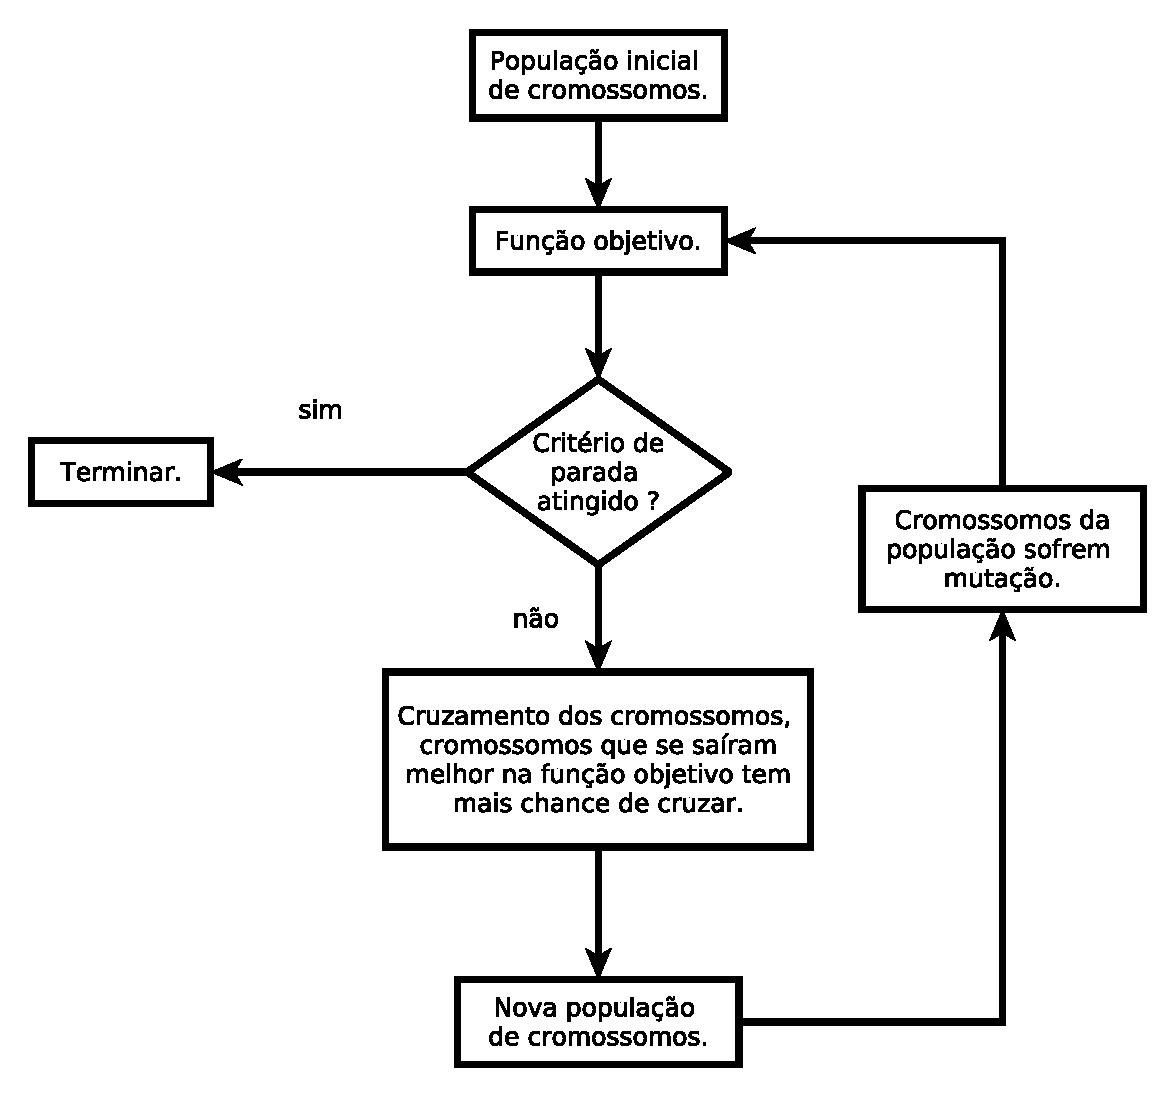
\includegraphics[scale=0.6]{imgs/diagramaAG.pdf}            
  \caption{Fluxograma ilustrando o conceito de algoritmos genéticos.}
  \label{fig:MostrandoOCruzamentoUniforme}
\end{figure}

\subsection{Angry Birds}
\label{sec:angryBirds}
O Angry Birds é um popular jogo de dispositivos portáteis (celulares) e computadores, a Figura \ref{fig:AngryBirds} mostra um \emph{screenshot} do jogo). O objetivo do jogo é jogar pássaros com um estilingue e acertar todos os porcos que estão no cenário com o menor número de pássaros possível, caso não seja possível se acertar todos os porcos com o número de pássaros que jogo fornece o jogador perde o jogo. A recepção de dados do ambiente para o agente é feita a partir de \emph{screenshots} tiradas do ambiente, o agente então, usando algoritmos de visão computacional, tem uma percepção completa sobre a situação do nível em que esta jogando.  

O ambiente para o jogo pode ser descrito como: 
\begin{itemize}
\item Completamente observável. Pois o \emph{framework} permite, através do uso de visão computacional, que o agente tenha um conhecimento sobre todas informações pertinentes ao ambiente para que ele tome suas escolhas. Entre as informações providas pelo \emph{framework} estão: Saber onde estão os inimigos, saber quais são estruturas do ambiente que são interativas e a que classe elas pertencem, saber o tipo de munição ("passarinho") que o agente possui.
\item  Não determinístico. Pois jogadas iguais produzem pontuações diferentes, o vídeo gravado (\url{https://youtu.be/epdZoGcC1EE}) pelo  autor deste trabalho mostra isto. Isto acontece por que possivelmente a simulação física de colisão e gravidade usa métodos de Monte Carlo, uma vez que estes métodos de simulação são mais baratos computacionalmente. Porem não foi achado nenhum documento no site do Angry Birds dizendo isto.
\item Sequencial. Por que conforme se atira pássaros nos porcos o ambiente vai mudando, por exemplo os blocos caindo, e o agente pode usar esta mudança a seu favor.
\item Estático. Isto depende do agente, no caso da implementação realizada neste trabalho o agente espera o ambiente se estabilizar entre os arremessos de pássaros. Por estabilizar se entende esperar que um novo pássaro só vai ser jogado após os blocos e pedras do ambiente já tiverem sé movido após o arremesso do pássaro anterior, isto é feito esperando-se 15 segundos entre cada arremesso de pássaro.  No entanto pode-se criar um agente que arremesse um pássaro seguido do outro, com uma pausa entre a jogadas tão pequena que enquanto um pássaro  ainda esta atingindo algo no ambiente (o que vai mudar o ambiente) outro já foi arremessado. 
\item Continuo. Pois existem infinitos ângulos e graus de força com que se pode arremessar os pássaros.
\item Agente único. 
\end{itemize}


\section{Modelagem do Angry Birds para algoritmos genéticos}
\label{sec:modelagem}
Para a modelagem se considerou que existem 3 tipos de genes, são eles:
\begin{itemize}
  \item Força, que diz com que força um pássaro é lançado do estilingue. Ele vai de  $0$ a $24$.
  \item Angulo,  que diz o angulo em que o pássaro é arremessado. Ele vai de  $0$ a $80$.
  \item Especial, que diz o tempo, em milissegundos, para ativação do especial a partir do momento em que o pássaro é lançado do estilingue. Ele vai de  $0$ a $2500$.
\end{itemize}

O número de genes dos cromossomos depende da quantidade de pássaros que o nível do jogo disponibiliza, pois cada pássaro deve possuir uma força de arremesso, um angulo de arremesso e um tempo para ativação de seu especial (este gene pode ser desconsiderado para o pássaro vermelho, por ele não possuir um especial). Para o nível 20, que foi o nível em que foram realizados os testes deste trabalho, são 15 genes para cada cromossomo. Isso acontece porque este  nível possui 5 pássaros amarelos. 

A função objetivo desta modelagem é um determinado nível do jogo Angry Birds, o 20 neste caso. Assim os cromossomos, de cada geração, arremessam um grupo de 5 pássaros (amarelos), depois dos arremessos cada cromossomo recebe do jogo uma nota por todos os seus arremessos. Como o objetivo deste trabalho é maximizar a função objetivo, ou seja obter a maior pontuação possível em um nível, os cromossomos que conseguem a maior pontuação são os mais aptos do ambiente. 

 Na modelagem deste trabalho, com o objetivo de tentar se preserva o máximo local, o melhor  cromossomo da geração atual sobrevive para a geração seguinte. Outra característica desta modelagem, para não ficar apenas no máximo local, é que a cada geração um cromossomo é gerado com genes aleatórios.
 
\section{Resultados}
Os dois principais resultados obtidos com este trabalho foram as taxas de aprendizagem e a eficiência alcançadas pelos métodos de seleção de cromossomos utilizados. Além disto foi feita uma comparação dos agentes treinados, em ambos os métodos de seleção, com um agente burro. 

\subsection{Taxas de aprendizagem} 
Neste trabalho se considerou a taxa de aprendizagem como sendo evolução da maximização da função objetivo descrita na Seção \ref{sec:modelagem}. Deste modo a taxa de aprendizagem seria a evolução da pontuação máxima obtida pela população de cromossomos conforme as gerações passam, cromossomos estes que o agente utiliza para jogar Angry Birds em um determinado nível. 

Uma outra medida, complementar a taxa de aprendizagem, seria a evolução da média da pontuação obtida pela população de cromossomos, utilizados pelo agente, conforme se avança nas gerações. 

As figuras \ref{fig:taxaAprendizagemTorneio} e \ref{fig:taxaAprendizagem2Torneio} mostram o \emph{plot} da taxa de aprendizagem e media de pontuação, para quando o agente é treinado com algoritmos genéticos que usam o método de seleção por torneio. A Figura \ref{fig:taxaAprendizagemRoleta}  mostra o \emph{plot} a taxa de aprendizagem e a Figura \ref{fig:mediaRoleta}  mostra o \emph{plot} da media de pontuação, quando o agente é treinado com algoritmos genéticos que usam o método de seleção por roleta. 
\begin{figure}[H]
  \center
  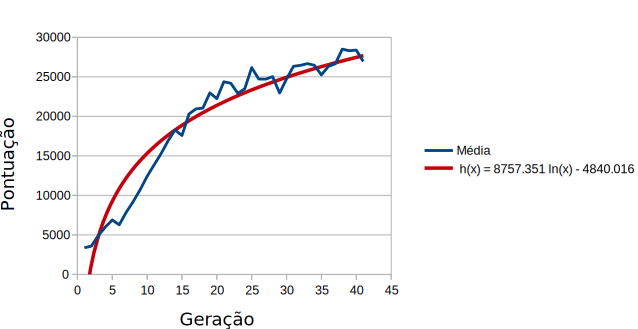
\includegraphics[scale=0.6]{imgs/plotTorneio.pdf}            
  \caption{Taxa de aprendizagem para o algoritmo genético que usa seleção por torneio, junto a função h(x) pela
qual foi ajustada.}
  \label{fig:taxaAprendizagemTorneio}
\end{figure}
\begin{figure}[H]
  \center
  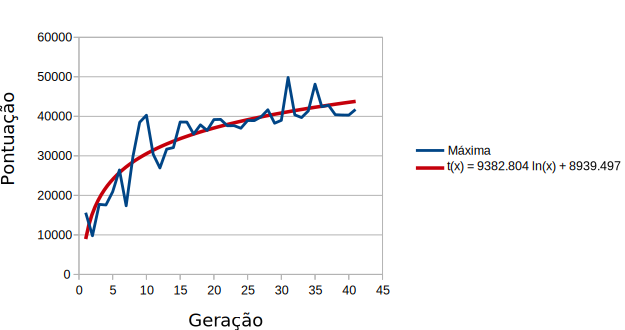
\includegraphics[scale=0.6]{imgs/plotTorneio2.pdf}
  \caption{Média da pontuação para o algoritmo genético que usa seleção por torneio, junto com a função t(x)
para qual foi ajustada.}
  \label{fig:mediaTorneio}
\end{figure}


\begin{figure}[H]
  \center
  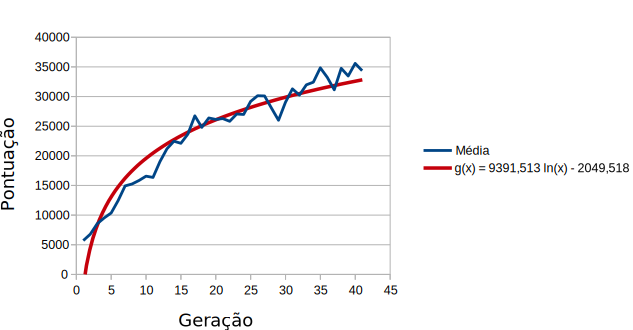
\includegraphics[scale=0.6]{imgs/plotRoleta.pdf}            
  \caption{Taxa de aprendizagem para o algoritmo genético que usa seleção por roleta, junto a função g(x) pela
qual foi ajustada.}
  \label{fig:taxaAprendizagemRoleta}
\end{figure}
\begin{figure}[H]
  \center
  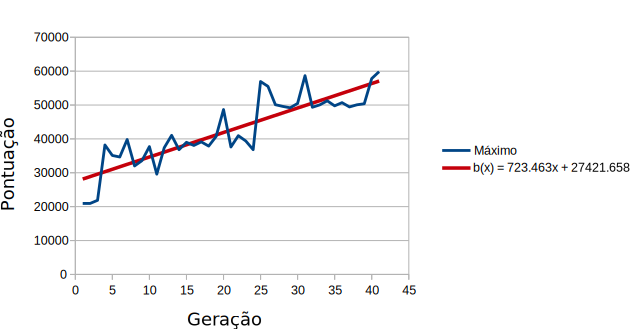
\includegraphics[scale=0.6]{imgs/plotRoleta2.pdf}
  \caption{Média da pontuação para o algoritmo genético que usa seleção por roleta, junto com a função b(x)
para qual foi ajustada.}
  \label{fig:mediaRoleta}
\end{figure}

Como pode-se ver o método da roleta, apresentou uma taxa de aprendizagem maior que o método do torneio. Isto pode ser visto matematicamente, derivando-se as funções $g(x)$ e $h(x)$  para as quais a taxa de aprendizagem de ambos os métodos foram ajustada. Uma vez que $g'(x)=$ e $h'(x)$ então $g(x)>h(x)$ pois $lim_{x \to \infty} \frac{g'(x)}{h'(x)}=0$ assim temos que a derivada para o método da roleta é uma derivada  que cresce mais rápido que a derivada do torneio.

Além disto o método da roleta também apresentou um melhor avanço na media de acertos da população de cromossomos, utilizados para jogar Angry Birds, conforme se passam as gerações. A demonstração matemática disto é análoga a mostrada no paragrafo anterior, basta substituir $g(x)$ por $b(x)$ e $h(x)$ por $t(x)$.

 Assim o método da roleta é melhor, do que o método  por torneio, em um ambiente de aprendizado como o descrito na Seção \ref{sec:angryBirds}.
 
\subsection{Comparação entre agentes treinados com o agente burro}
Para esta comparação foi adotado o critério de criar três agentes e  comparar a pontuação que eles obtém. Um dos agentes  é criado com  o melhor cromossomo gerado pelo método da roleta, o outro agente é criado com o melhor cromossomo gerado pelo método do torneio  e o ultimo agente é o agente ``burro''.

Para obter-se a pontuação a partir do agente ``burro'' se jogou o nível 20 do  Angry Birds com ele 10 vezes, a partir disso foi extraído uma média e um desvio padrão da pontuação das jogadas, além disto também foi considerado a pontuação máxima e  miníma que o agente ``burro'' conseguiu no jogo como métricas importantes. Para os agentes criados a partir dos cromossomos também se utilizou o mesmo critério que o agente ``burro'' utilizou para se extrair as métricas da pontuação ou seja,  cada um dos agentes jogou 10 vezes o nível 20 do jogo. Isto foi feito por que conforme dito na Seção \ref{sec:angryBirds} o ambiente em que os agentes foram treinados possui um certo grau de não determinismo. 

A Tabela \ref{tab:comparacaoDosAgentes} apresenta as medidas, desvios padrões, pontuação máxima e pontuação miníma que os dos cromossomo selecionados junto com o agente burro obtiveram.
\begin{table}[h]
  \small
  \begin{tabular}{|L{5cm}|l|l|l|l|}%
    \hline                                                                    
    \textbf{} & \textbf{Média} & \textbf{Desvio Padrão} & \textbf{Máximo} & \textbf{Mínimo} \\ \hline 
    Agente burro & 17341 & 2688.633 & 21390 & 13720 \\ \hline
    Agente criado  pelo cromossomo obtido pelo método da roleta & 31049 & 9236.183 & 47270 & 12240 \\ \hline
    Agente criado pelo cromossomo obtido pelo método do torneio & 28229 & 8720.646 & 49670  & 19950 \\ \hline
  \end{tabular}
  \caption{Média, desvio Padrão, máximo e mínimo da pontuação que o agente burro e os agentes criados pelos cromossomos, obtidos pelos métodos roleta e torneio, conseguem no Jogo Angry Birds. Estes dados foram obtidos a partir de 10 partidas realizadas por cada um dos agentes criados.}
  \label{tab:comparacaoDosAgentes}    
\end{table}
\section{Conclusão}
Neste trabalho foi feita uma comparação entre dois métodos para a seleção de cromossomo em algoritmos genéticos. Usando-se como base para comparação o ambiente do jogo Angry Birds.  As analises mostram que o método de seleção por roleta se saiu melhor para o ambiente do jogo. 

Também foi realizada uma comparação de pontuação entre os agentes criados pelos melhores cromossomos obtidos por ambos os métodos de seleção, de algoritmos genéticos, com um agente burro disponibilizado pelo site IA-Birds. Ambos os agentes criados a partir dos cromossomos foram melhor que o agente burro. O que mostra que algoritmos genéticos são um bom método de IA para resolução de problemas como descritos pelo ambiente do Angry Birds.
\bibliography{bibliografia}
\bibliographystyle{plain}
\end{document}

\message{ !name(sumarioExecutivo.tex) !offset(-151) }

